%%%%%%%%%%%%%%%%%%%%%%%%%%%%%%%%%%%%%%%%%%%%%%%%%%%%%%%%%%%%%%%%%%%%%%%%%%%%%%%
% main.tex, arXiv version.
%%%%%%%%%%%%%%%%%%%%%%%%%%%%%%%%%%%%%%%%%%%%%%%%%%%%%%%%%%%%%%%%%%%%%%%%%%%%%%%

\documentclass[11pt]{article}

\usepackage[letterpaper, margin=1in]{geometry}
\usepackage[utf8]{inputenc}
\usepackage[T1]{fontenc}
\usepackage{lmodern}
\usepackage{hyperref}
\usepackage{url}
\usepackage{booktabs}
\usepackage{amsfonts}
\usepackage{nicefrac}
\usepackage{microtype}
\usepackage{xcolor}
\usepackage{graphicx}
\graphicspath{{./}{figures_xfer/}{../../figures/}{../../}}
\usepackage{subcaption}
\usepackage{amsmath}
\usepackage{amssymb}
\usepackage{mathtools}
\usepackage{natbib}
\usepackage{authblk}
\usepackage{algorithm}
\usepackage{algorithmic}
\usepackage[capitalize,noabbrev]{cleveref}

\hypersetup{
    colorlinks=true,
    linkcolor=blue!60!black,
    citecolor=blue!60!black,
    urlcolor=blue!60!black,
}

\title{Fully Autonomous Continual Learning and Knowledge Transfer\\ via Cortex-Inspired Neural Assemblies}

\author[1]{*}
    %*Kevin L. McKee, Yicong Zheng, Zacharie Bugaud, Thomas Miconi}
\affil[1]{Astera Institute}

\date{}

\begin{document}

\maketitle

% =====================================================================
\begin{abstract}
Continual learning requires both parameter isolation to protect task-specific computation, and parameter reuse to transfer useful computation to later tasks. We introduce Functional Task Networks (FTNs), a unified mechanism of continual learning and knowledge transfer modeled after several properties of the mammalian neocortex. An FTN is formulated as a large, distributed, stochastic mixture of experts in which a sparse routing mask is computed at inference time over a small support sample of input-output pairs. Per-batch reconfiguration during training, together with mask-overlap-filtered replay, shapes a basis of overlapping, partially trained subnetworks. Unrelated tasks route through mostly separate assemblies, related tasks overlap on shared components. On block-sequentially trained continual learning and knowledge transfer tasks including shuffled MNIST for concept shift, Permuted MNIST for domain shift, and Rotated MNIST for knowledge transfer, FTN retains solutions nearly as well as disjoint-mask isolation and attains the lowest pre-update head-start loss among matched-architecture comparators. The learned mask-overlap geometry tracks the known concept-sharing structure where available. We show experimentally that under correlated concept shift, support-set mask reconfiguration is necessary even for retention. Under domain shift, the distributed bank with replay is sufficient to handle retention without the configurer. Forward transfer, or head-start, and backward transfer, are also contributed by support-set mask configuration. We further implement FTN-LoRA, a bank of Low Rank Adaptation modules on a frozen Qwen2.5-1.5B backbone, and test over a six-task multilingual classification stream, demonstrating minimal forgetting and positive backward transfer in a scaled setting.
\end{abstract}

% =====================================================================
\section{Introduction}\label{sec:intro}

For continual learning in neural networks, shared parameters let a new task reuse representations learned from earlier tasks, but the same shared parameters can be overwritten by later gradients, producing catastrophic forgetting \citep{mccloskey1989catastrophic,french1999catastrophic}. Parameter isolation methods protect earlier computations by assigning tasks to separate subnetworks \citep{mallya2018packnet,serra2018overcoming,wortsman2020supermasks}, but isolation weakens forward transfer because new tasks cannot easily recruit useful structure from old ones. A central question for general continual learning solutions is therefore how a model might automatically modulate between isolating and sharing its parameters.

\paragraph{Concept and domain shift.}
Continual-learning benchmarks differ in \emph{what} changes between tasks. Under \emph{domain shift} the input distribution changes while the labeling rule remains broadly compatible. The most generic way to prevent forgetting under domain shift is shuffled replay-based methods \citep{lopez2017gradient,chaudhry2018efficient,buzzega2020dark}, in which data from previous tasks are mixed in training minibatches. The gradients over the tasks are averaged, so no single task dominates all of the weight updates. Under \emph{concept shift} the labeling rule or output function itself changes, so the same input must be mapped to different targets in different tasks. Methods like Elastic Weight Consolidation (EWC) and Synaptic Intelligence \citep{kirkpatrick2017overcoming,zenke2017continual} address domain shift but not concept shift. Penalizing drift on parameters that \emph{need} to compute different functions on different tasks only blocks learning. Naive replay similarly fails because two replayed labels for the same input contradict each other unless replay is routed through different subnetworks.

\paragraph{Block-sequential training.}
Block sequential training presents a maximally difficult regime for retention than i.i.d.\ minibatching: each long stretch of updates is dominated by one task at a time, intensifying forgetting on other tasks. It is also the schedule of most realistic continual deployments (sequential adapter installation, on-the-job fine-tuning, sliding-window streams). We specifically target this training regime as a necessary part of the continual learning problem definition.

\paragraph{Functional Task Networks.}
We introduce Functional Task Networks (FTNs), a support-set-conditioned routing mechanism for continual learning without task identity. FTN uses a large bank of small but deep networks to learn modular but distributed task representations. During both training and inference, FTN selects a sparse assembly for each minibatch by optimizing a binary top-k mask to minimize loss with respect to a small labeled support set. This gives a single mechanism for both parameter isolation and reuse: unrelated tasks can be routed through mostly different assemblies, while related tasks can overlap on components that carry useful computation. In this paper, we evaluate whether this mechanism produces the intended trade-off: retention under block-sequential training and concept shift, forward transfer before any update on a new task, and mask-overlap structure that reflects task relatedness when such structure is known. We show that FTN occupies a middle regime between full parameter sharing and fixed disjoint masks, retaining most of the protection of isolation while enabling recombination that fixed task masks cannot provide.

\paragraph{Biological motivation.}
FTN is motivated by several features of neocortical computation that suggest a route to sparse, reusable, and partially overlapping task representations. Sparsification via top-$k$ masking has previously served as an abstraction for the effects of inhibitory competition among neurons\citep{yang2019task,cichon2015branch,mongillo2018inhibitory,rolls2010attractor,khona2022attractor,amari1977dynamics,maass2000computational,douglas2004neuronal}. Our choice to use a large number of deep networks with low-dimensional output is based on the dendritic model of pyramidal neurons, which can be characterized as deep, multilayer networks\citep{poirazi2003pyramidal,poirazi2020illuminating,beniaguev2021single}.

We also draw on a statistical property of cortical representations: task-relevant activity is distributed across populations and partially redundant, rather than localized to single reliable units \citep{georgopoulos1986neuronal,averbeck2006neural,cohen2011measuring}, while individual cortical neurons are variable across trials and only partially reliable \citep{tolhurst1983statistical,softky1993highly,shadlen1998variable,faisal2008noise,churchland2010stimulus,goris2014partitioning}. Algorithmically, this motivates using a large population of small subnetworks whose contributions are individually weak but heterogeneous, and whose training histories differ across tasks. A new task can then be configured by selecting an assembly from many partially trained units, allowing useful computation before any further weight update. In this view, transfer arises not from retrieving a single stored expert, but from recombining a distributed population of imperfect, task-shaped components.

\paragraph{Contributions.}
Our contribution is to study continual learning as a support-conditioned routing problem: at each training and evaluation step, a small labeled support batch replaces explicit task identity as the evidence used to infer which computation should be active. FTN implements this idea by optimizing a sparse binary assembly mask over a large bank of independently parameterized subnetworks while holding model weights fixed during configuration. This gives a single mechanism for isolation and transfer: masks can separate tasks with incompatible input-output rules, but can also overlap when the support set indicates reusable computation. Empirically, we show that per-batch mask reconfiguration during training is the key ingredient: it creates a broad basis of partially trained subnetworks that later tasks can recombine, producing lower pre-update head-start loss than fixed parameter-isolation and retrieval baselines while retaining most of their protection against forgetting. Across controlled concept- and domain-shift benchmarks, FTN therefore occupies a middle regime between full sharing and disjoint task masks: it does not assume task identity, but it does assume labeled functional evidence from the current task, and its goal is to convert that evidence into task-appropriate reuse.

% =====================================================================
\section{Related work}\label{sec:related}

The first class of related models focus primarily on retention of prior solutions. Parameter-isolation methods (PackNet \citep{mallya2018packnet}, HAT \citep{serra2018overcoming}, SupSup \citep{wortsman2020supermasks}) assign tasks to disjoint parameter subsets; regularizers (EWC \citep{kirkpatrick2017overcoming}, Synaptic Intelligence \citep{zenke2017continual}) penalize drift on parameters important for earlier tasks; replay methods (GEM/A-GEM \citep{lopez2017gradient,chaudhry2018efficient}, iCaRL \citep{rebuffi2017icarl}, DER++) use stored exemplars. These target retention; they have no explicit mechanism for forward transfer.

Other methods target both retention and knowledge transfer. Progressive Networks \citep{rusu2016progressive} dedicate a fresh column per task with lateral connections to prior columns, attaining perfect retention at linear-in-tasks parameter cost. PathNet \citep{fernando2017pathnet} searches paths through a fixed module bank and reuses modules via path overlap, the closest conceptual analog to FTN. Modular networks with task-driven priors \citep{veniat2021mntdp} make module-reuse-vs-grow explicit; meta-learning approaches such as OML \citep{javed2019oml} target both axes through the meta-objective. We position FTN inside this family: a parallel-bank architecture with a binary support-set-derived mask that uses the same optimization to control isolation and transfer.

Among knowledge transfer methods, the most relevant to FTN are those that use inference-time support-set to determine the router state. Sparse expert models \citep{shazeer2017outrageously,fedus2022switch} and conditional channel-gated networks \citep{abati2020conditional} learn gates over subnetworks. More directly relevant, a family of methods uses a labeled support set to infer task identity or pick from a bank of stored task models: supermask retrieval in SupSup \citep{wortsman2020supermasks}, prompt-pool selection in L2P and DualPrompt \citep{wang2022learning,wang2022dualprompt}, and learned routers on support-set features. This is the central comparator class.

Finally, Top-$k$ routing requires optimization through a discrete constraint; we compare a sigmoid relaxation, an annealed straight-through estimator \citep{bengio2013estimating}, and a Gumbel-Sigmoid / Concrete relaxation \citep{jang2017categorical,maddison2017concrete} as three candidate methods for determining the routing mask.

% =====================================================================
\section{Method}\label{sec:method}

\paragraph{Architecture.}
An FTN contains $H$ independent scalar-output ``neurons'', i.e. subnetworks $z_j=f_j(x)$. A binary mask $m\in\{0,1\}^H$ with $\|m\|_0=k$ selects an active subset of the networks, and a linear readout produces
\[
  \hat{y} = W_\mathrm{out}\,(\mathrm{Dropout}(z)\odot m).
\]

The model tested here uses $H=8192$ neurons, each an MLP with $L=8$ hidden layers of width $8$, dropout $p=0.2$. Of these, $k=512$ neurons were active at a time. All architecturally-matched baselines use the same parallel bank. The bank of neurons is deliberately wide relative to the per-task budget. Any individual neuron is unreliable (it may have been trained on an unrelated task or be inactive on the current input) so the configurer aggregates a sparse subset of noisy units. The combinatorially large pool of partially trained subnetworks is what the reconfiguration inner loop recombines into a transfer solution on a new task, rather than a small number of curated experts.

A configurer $C$ receives the current model and a labeled support batch and returns a hard top-$k$ mask after $S$ inner steps with model weights fixed. We compare Sigmoid, AnnealSTE, and Gumbel-Sigmoid forms; AnnealSTE with $S{=}30$ was chosen as the default after performing sweeps across each of the three methods and values of $S$ (full details in \cref{app:impl}).

To train neurons shared across tasks, each step draws a $(x,y,m)$ triple from a $200$-slot buffer filtered by mask overlap: a stored entry is admitted when its mask overlaps the current mask moderately, $\rho \in (0.2, 0.8]$. Entries with $\rho \le 0.2$ share too little mass to interfere, while entries with $\rho > 0.8$ are likely already trained by the current or proximal minibatches. Filtered replay therefore spends replay supervision only on the overlapping parameters, targeting task interference directly, while the disjoint complement is protected by mask gating. As a comparison, matched-memory uniform-random sampling (NoMask\,+\,ER in \cref{sec:results_mnist}) ablates the contribution of the filter.

\paragraph{FTN training and evaluation procedure.}
\Cref{alg:ftn} summarizes the full FTN training and evaluation loop, combining the configurer, the mask-overlap-filtered replay, and the support-set-driven evaluation protocol. The same configurer $C$ is used at every training step and at evaluation time; the only difference between training and evaluation is whether the model parameters $\theta$ receive a gradient step.

\begin{algorithm}[t]
\caption{Functional Task Networks: training and reconfig evaluation}
\label{alg:ftn}
\begin{algorithmic}[1]
\REQUIRE Tasks $\{\mathcal{T}_t\}_{t=1}^{T}$ arriving block-sequentially; bank of $H$ subnetworks $\{f_j\}$ with parameters $\theta$; readout $W_\mathrm{out}$; active budget $k$; configurer $C$ with $S$ inner steps; replay buffer $\mathcal{B}$ of capacity $N_\mathcal{B}$; replay overlap window $(\rho_\mathrm{lo}, \rho_\mathrm{hi}]$; support size $n_s$
\STATE Initialize $\theta$, $W_\mathrm{out}$, $\mathcal{B}\leftarrow\varnothing$
\FOR{task $t=1,\dots,T$}
    \STATE Reset optimizer state for $(\theta, W_\mathrm{out})$
    \FOR{each training minibatch $(x, y) \sim \mathcal{T}_t$}
        \STATE Draw support batch $(x_s, y_s)\sim \mathcal{T}_t$ of size $n_s$
        \STATE \textbf{// Mask configuration with $\theta$ frozen}
        \STATE Initialize mask logits $m_0$; \textbf{for} $s=1,\dots,S$ \textbf{do} $m_s \leftarrow$ configurer step $C(m_{s-1}; x_s, y_s, \theta)$
        \STATE $m_\mathrm{cur} \leftarrow \mathrm{TopK}(m_S, k) \in \{0,1\}^H$
        \STATE \textbf{// Mask-overlap-filtered replay}
        \STATE Sample $(x_r, y_r, m_r)$ uniformly from $\{(x', y', m')\in\mathcal{B} : (m'\!\cdot m_\mathrm{cur})/k \in (\rho_\mathrm{lo}, \rho_\mathrm{hi}]\}$
        \STATE \textbf{// Gradient step through the active mask, current plus replay}
        \STATE $\mathcal{L} \leftarrow \mathrm{loss}(W_\mathrm{out}(z(x)\odot m_\mathrm{cur}), y) + \mathrm{loss}(W_\mathrm{out}(z(x_r)\odot m_r), y_r)$
        \STATE Update $(\theta, W_\mathrm{out})$ with $\nabla \mathcal{L}$
        \STATE Optionally insert $(x, y, m_\mathrm{cur})$ into $\mathcal{B}$ (evict oldest if $|\mathcal{B}|=N_\mathcal{B}$)
    \ENDFOR
\ENDFOR
\STATE \textbf{Evaluation (reconfig protocol).} Given any target task $t^\star$ and an unlabeled query, draw a labeled support batch from $\mathcal{T}_{t^\star}$, run the configurer for $S$ inner steps with $\theta$ frozen to obtain a mask $m^\star$, and predict $\hat{y} = W_\mathrm{out}(z(x)\odot m^\star)$. Task identity is never disclosed.
\end{algorithmic}
\end{algorithm}

% =====================================================================
\section{Experiments}\label{sec:experiments}

\paragraph{Training and evaluation.}
In each of the following experiments, tasks arrive in contiguous blocks. Before every forward pass of FTN, its configurer selects a mask on the current minibatch, then the model updates through that mask only, with one mask-filtered replay sample drawn as described above. At evaluation, all models under comparison receive a small labeled support set from a target task, and for evaluating retention and transfer, a disjoint held-out batch from the same task. The task identity is never disclosed. The configurer selects a mask using the support set, and all metrics are computed on the held-out batch. For FTN, we refer to this as the \emph{reconfig} protocol. For diagnostics only, we also report a \emph{stored} protocol that reuses a saved training mask and therefore acts as a task-identity oracle.

\paragraph{Comparator suite.}
Seven comparators run on the same parallel-MLP backbone and support-set evaluation protocol. \emph{NoMask} (naive sequential fine-tuning), \emph{NoMask\,+\,ER} (uniform-random replay buffer matched in capacity to FTN's filtered buffer), and \emph{FixedMask} (deterministic disjoint per-task blocks, task identity at eval) are the full-sharing/replay/oracle-isolation baselines. \emph{SupSup} \citep{wortsman2020supermasks} freezes a randomly initialized parallel bank and learns a per-task score vector and readout, evaluated by support-set retrieval over stored masks. \emph{Progressive Networks} \citep{rusu2016progressive} use disjoint per-task $k$-blocks on the same bank with old columns frozen and lateral access from prior columns into the new readout, evaluated by support-set retrieval over the stored cumulative-column masks. \emph{FixedMask\,+\,Router} is the simpler PackNet-style retrieval baseline; \emph{FTN\,+\,Router} (FTN training, retrieval at eval) asks whether the FTN inner loop beats simple retrieval over the FTN-trained bank.

Several standard continual-learning methods, including EWC, SI, LwF, GEM/A-GEM, DER++, HAT, and PackNet, optimize primarily for retention under different architectural and evaluation assumptions than the support-conditioned routing setting studied here. In particular, many assume explicit task identity, fixed task boundaries, or architectures that do not naturally map onto FTN's large sparse-bank setting. Rather than presenting potentially misleading reimplementations under mismatched constraints, we construct architecture-matched controls that isolate the underlying mechanisms most relevant to FTN: replay-based full sharing (NoMask+ER), oracle parameter isolation (FixedMask), and support-set retrieval over isolated subnetworks (FixedMask+Router). PathNet, MNTDP, and L2P/DualPrompt require a non-MLP backbone and are deferred to the LoRA-bank instantiation. Per-benchmark mean$\pm$std tables are in \cref{app:revision_tables}.


\subsection{Benchmarks and metrics}\label{sec:setup}
An class-label generating function of arbitrary difficulty for artificial neural networks can be generated by composing sinusoids of random input-conditioned frequencies. The \emph{synthetic} task family has $T{=}12$ binary classification tasks in $d{=}2$ generated from a fixed-encoder sinusoidal mixture over $C{=}6$ latent concept components: $x \sim \mathcal{N}(0, I_d)$, $\tilde z(x; t) = \sin\!\bigl(f\,(W_\mathrm{enc} x \odot m_t)\bigr)\odot m_t$, $y(x;t)=\mathbb{1}[\sum_l \tilde z_l > 0]$, with $f{=}8$ and $m_t\in\{0,1\}^L$ a binary task-component selector. The \emph{correlated} variant has $m_t$ select two of $C{=}6$ components (one of $\binom{6}{2}{=}15$ pairs, uniquely per task), so each component is shared by exactly two tasks; the \emph{orthogonal} variant uses $C{=}2T{=}24$ components partitioned into disjoint pairs (zero off-diagonal sharing). \Cref{fig:tasks} shows three example tasks mapping $(x_0, x_1)$ to $y$.

The MNIST suite~\citep{lecun1998mnist} spans concept and domain shift: \emph{shared-shuffle MNIST} (6 tasks) gives each task a digit-to-label permutation that is the union of two component sub-permutations, exposing ground-truth concept overlap; \emph{Permuted MNIST} and \emph{Rotated MNIST} (10 tasks each) are domain-incremental, applying a fixed random pixel permutation or a fixed rotation in equal steps from $0$ to $180^\circ$. Each MLP cell trains 1{,}000 Adam steps per task at lr $3{\times}10^{-4}$, train minibatch size $256$, and optimizer-state reset at task boundaries.

\begin{figure}[!ht]
\centering
\includegraphics[width=0.85\textwidth]{tasks.png}
\caption{Three example tasks from the correlated synthetic family: binary decision surface over the 2-D input $x$, points colored by class $y$. Tasks share latent components; boundaries share gross structure but differ in orientation and high-frequency interior, the concept overlap FTN's mask geometry is designed to recover.}
\label{fig:tasks}
\end{figure}

We report (1) accuracy (ACC) as the average classification accuracy across all tasks trained block-sequentially, (2) forgetting measure (FM) \citep{chaudhry2018efficient} i.e, the loss retroactively contributed by new tasks, and (3) backward transfer (BWT) \citep{lopez2017gradient} on the lower-triangular performance matrix under the reconfig protocol; (4) \emph{head-start loss} is the loss on a held-out batch from a new task after support-set mask configuration but before any weight update on that task, and lower values indicate stronger forward transfer. On the synthetic and shared-shuffle MNIST families, where ground-truth overlap is known, $r_{\mathrm{share}}$ is the Pearson correlation between off-diagonal entries of the row-normalized mask-overlap matrix and the ground-truth concept-sharing matrix.


\section{Results}


\subsection{Synthetic concept sharing}\label{sec:results_synthetic}

The correlated synthetic family is the only benchmark where ground-truth concept overlap is known by construction, so retention, forward transfer, and the recovered routing geometry can all be checked against a defined target. \Cref{tab:revision_synthetic} shows that unmasked sequential training collapses ($\mathrm{FM}{=}0.396$ for NoMask) and matched-memory random replay only partly recovers ($\mathrm{ACC}{=}0.65$). The four parameter-isolation methods reach $\mathrm{FM}{=}0$ to within sample noise (by construction for three; within $0.03$ for FTN despite no provided task identities), so retention does not separate the masked methods. The differences are on the other axes.

ACC reflects how much each isolation strategy lets the model learn: SupSup at $0.768$ is bottlenecked by its frozen random backbone, Progressive and FixedMask reach the oracle's $\approx 0.95$ by allocating fresh trained capacity per task, and FTN sits a few points below ($0.92$) because its bank weights are shared rather than partitioned.

Head-start loss measures how well the active subnetwork is already configured for a new task before any weight update (averaged across tasks in the sequence): FTN at $0.40$ is below every other comparator, including Progressive ($1.42$, ${\sim}3.5\times$) and SupSup ($0.66$).
Interestingly, FTN\,+\,Router reproduces FTN's number ($0.394$ vs.\ $0.399$) while the same retrieval on top of FixedMask, SupSup, or Progressive cannot.
For the router version, which retrieved masks from an explicit memory, the per-batch reconfiguration during \emph{training} is what populates that memory with a large variety of partly-trained overlapping subnetworks. It follows from these results that taking the $\arg\min$ of the loss over that bank is a viable but much more computationally expensive alternative to the reconfiguration's gradient-based search, which only used 30 steps.

The no-replay ablation raises FM about seven-fold (to $0.195$) and drops ACC to $0.78$, which localizes retention to the filtered-replay channel that protects shared neurons. Random per-batch masks (FTN training pipeline, configurer replaced by a fresh random $k$-of-$H$ mask each step) retain and transfer substantially worse than FTN under correlated concept shift, with ACC dropping from $0.919$ to $0.774$, FM rising from $0.029$ to $0.119$, and head-start loss rising from $0.399$ to $1.194$, showing that stochastic sparse-bank training plus replay is insufficient when tasks share latent components and that the support-conditioned configurer is necessary to route around the resulting cross-task mask collisions.

% Auto-generated by experiments/generate_revision_tables.py.
\begin{table}[t]
\centering
\small
\caption{Correlated synthetic family (12 tasks) under the reconfig (no-task-identity) protocol. Mean$\pm$std over 5 seeds. Higher ACC and BWT, lower FM and head-start (HS) loss, are better.}
\label{tab:revision_synthetic}
\begin{tabular}{lllll}
\toprule
Method & ACC$\uparrow$ & FM$\downarrow$ & BWT$\uparrow$ & HS$\downarrow$ \\
\midrule
NoMask (naive seq.) & $0.607 \pm 0.019$ & $0.396 \pm 0.017$ & $-0.396 \pm 0.017$ & $2.868 \pm 0.339$ \\
NoMask + ER (random replay) & $0.651 \pm 0.029$ & $0.165 \pm 0.011$ & $-0.164 \pm 0.010$ & $1.074 \pm 0.081$ \\
FixedMask (oracle ID at eval) & $0.948 \pm 0.022$ & $0.000 \pm 0.000$ & $0.000 \pm 0.000$ & $0.702 \pm 0.003$ \\
FixedMask + retrieval router & $0.948 \pm 0.021$ & $0.000 \pm 0.000$ & $0.000 \pm 0.000$ & $0.702 \pm 0.004$ \\
FTN (ours) & $0.919 \pm 0.020$ & $0.029 \pm 0.007$ & $-0.021 \pm 0.015$ & $0.399 \pm 0.064$ \\
FTN, random masks (ablation) & $0.774 \pm 0.089$ & $0.119 \pm 0.042$ & $-0.113 \pm 0.045$ & $1.194 \pm 0.198$ \\
FTN + retrieval router & $0.904 \pm 0.028$ & $0.045 \pm 0.008$ & $-0.043 \pm 0.011$ & $0.394 \pm 0.078$ \\
FTN, no replay & $0.780 \pm 0.036$ & $0.195 \pm 0.028$ & $-0.192 \pm 0.031$ & $0.521 \pm 0.064$ \\
\bottomrule
\end{tabular}
\end{table}


\paragraph{16-task retention and transfer}\label{null_vs_full}

\Cref{fig:null_vs_full} contrasts the unmasked control (no routing, full network capacity exposed to every task) with the full FTN method on the same task family, same seed, and otherwise identical pipeline. Both panels are $16\times 16$ task-vs-task evaluation matrices obtained by training each model sequentially on $16$ orthogonal tasks from the synthetic data generator and then evaluating the resulting model on each task's held-out batch at every intermediate checkpoint.

\Cref{fig:null} is the \emph{null} result, with no masking and full network capacity. Only the diagonal displays high accuracy: the model only performs well on the task it has just finished training, with no retention (lower scores /redder color in the lower triangle, indicating that prior tasks have been overwritten) and no forward transfer (the upper triangle is also red, indicating that the pre-training on earlier tasks contributes nothing to later tasks). \Cref{fig:full} is the complete FTN method on the same $16$-task sequence. The lower triangle shows uniformly high scores that are close to those on the diagonal, i.e., near-perfect retention of every prior task after later tasks have been learned. The upper triangle is also substantially better than the null result, showing a large amount of forward transfer which improves as more tasks are introduced.

\begin{figure}[!ht]
\centering
\begin{subfigure}[b]{0.48\textwidth}
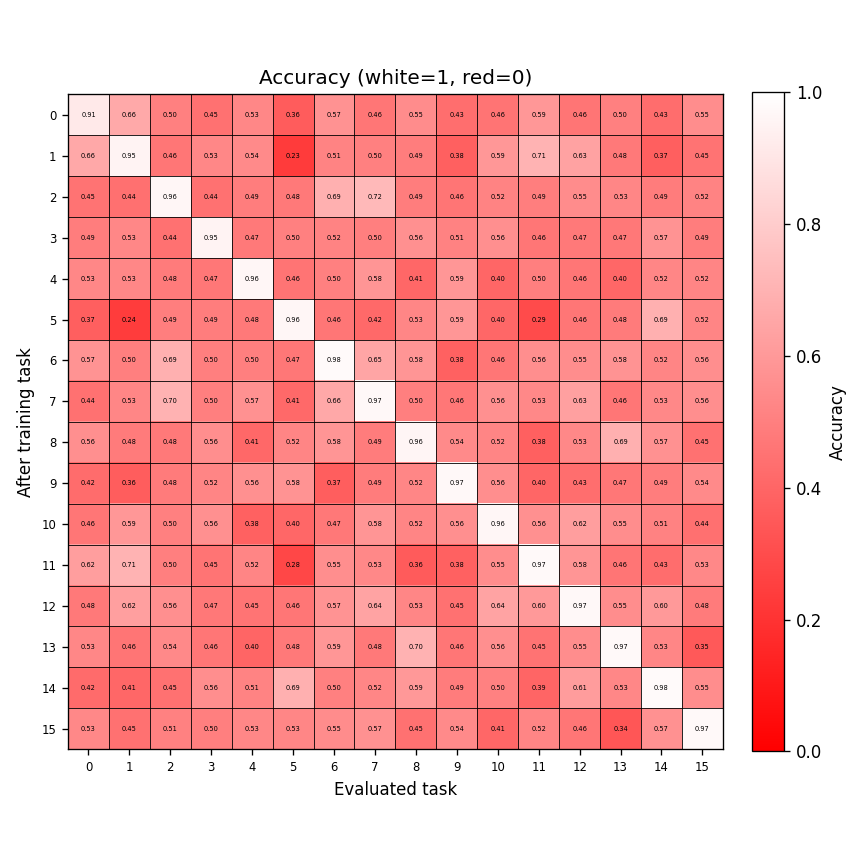
\includegraphics[width=\textwidth]{xfer_p1_mtl_null_orth.png}
\caption{Null result with the full network capacity but no masking or replay.}
\label{fig:null}
\end{subfigure}\hfill
\begin{subfigure}[b]{0.48\textwidth}
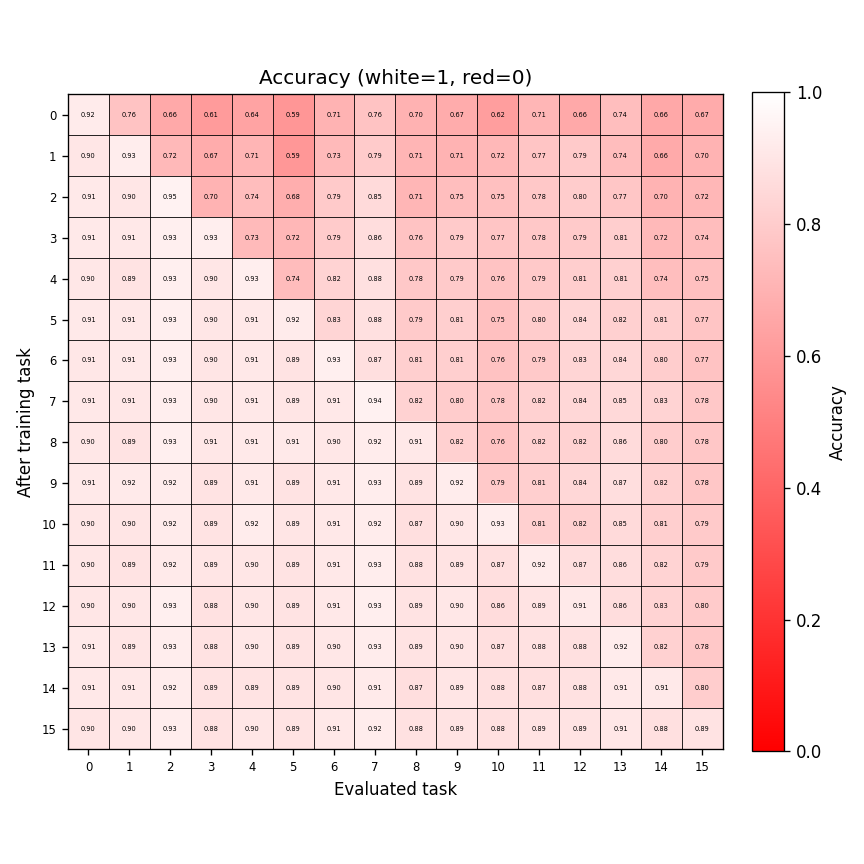
\includegraphics[width=\textwidth]{xfer_p1_mtl_eval_full_orth.png}
\caption{Full method: complete FTN with support-conditioned routing and mask-filtered replay.}
\label{fig:full}
\end{subfigure}
\caption{Per-task evaluation matrices on the $16$-task synthetic sequence, same seed and same pipeline modulo the FTN mechanism. Rows index training task; columns index evaluation task. The null exposes the bare-network behavior under block-sequential training; the full method recovers both retention and forward transfer on the same task family, with forward transfer improving as more tasks are introduced.}
\label{fig:null_vs_full}
\end{figure}

In \Cref{fig:null_vs_full}, the task are generated to be orthogonal, i.e., not share any data-generating function components, but the null results show that some chance correlation between tasks is present, and the full results show that the model can exploit such chance correlations in its forward knowledge transfer. Where task-invariant representations did not exist, the distributed and stochastic training of the network produced a large repertoire of partially-trained task bases that nonetheless allowed rapid construction of solutions on each new task.

\paragraph{Sparsity, support size, and the orthogonal control.}
Three diagnostic sweeps are summarized here; full tables and figures are in \cref{app:ablation_tables,app:sec_exp}. (i)~The top-$k$ budget controls how much overlap is possible: sweeping $k\in\{512,128,32,8\}$ reveals an isolation-transfer trade-off. FM falls from $0.056$ at $k{=}512$ to $0.032$ at $k{=}32$ while head-start rises from ${\approx}0.42$ to ${\approx}0.60$; sharing fidelity peaks at moderate sparsity ($r_{\mathrm{share}}{=}0.624$ at $k{=}32$). (ii)~Support-set size affects transfer more than retention: shrinking the support from $256$ to $4$ raises head-start from $0.425{\pm}0.080$ to $1.339{\pm}0.095$ while FM stays at or below $0.060$ and ACC at $0.86$ to $0.89$. (iii)~The orthogonal variant, which removes latent sharing while preserving the task format, raises FTN head-start from $0.423{\pm}0.077$ to $0.568{\pm}0.045$ with low forgetting in both regimes; $r_{\mathrm{share}}$ is zero by construction for the orthogonal task family.

\paragraph{Recovered sharing geometry.}
\Cref{fig:sharing_and_bwt} compares the ground-truth sharing matrix with the row-normalized neuron-sharing matrix for a high-fidelity AnnealSTE configuration ($S{=}40$, $r_{\mathrm{share}}{=}0.617$; the primary sweep reaches $0.622$). The recovered matrix is not binary, but its high-overlap regions align with the concept-sharing pattern. BWT stays close to zero across the 18 primary-search configurations, ranging from $-0.061$ to $+0.005$, against $-0.392$ for NoMask on synthetic and $-0.656$ on MNIST.

\begin{figure}[t]
\centering
\begin{subfigure}[b]{0.4\textwidth}
\includegraphics[width=\textwidth]{synthetic/sharing_gt.pdf}
\caption{Ground-truth.}
\end{subfigure}\hfill
\begin{subfigure}[b]{0.4\textwidth}
\includegraphics[width=\textwidth]{synthetic/sharing_model_AnnealSTE_b40.pdf}
\caption{Model, AnnealSTE $S{=}40$, $r_{\mathrm{share}}{=}0.617$.}
\end{subfigure}
\caption{Recovered task structure on the correlated synthetic family. Off-diagonal entries $S[i,j]$ count neurons (left) or concept components (right) shared between tasks $i\ne j$; the diagonal counts neurons / components used only by task $i$. $r_{\mathrm{share}}$ is computed on row-normalized off-diagonal entries.}
\label{fig:sharing_and_bwt}
\end{figure}


\subsection{MNIST concept and domain shift}\label{sec:results_mnist}
MNIST provides a non-synthetic validation that the transfer pattern is not an artifact of the sinusoidal generator. \Cref{tab:mnist_suite} compresses the three variants. On shared-shuffle MNIST (concept shift), random replay fails as predicted, NoMask and NoMask+ER collapse relative to the masked methods and have severe forgetting, while FTN retains within $0.023$ FM and has much lower head-start loss than all isolation/retrieval baselines ($0.562$ vs.\ $2.309$ for FixedMask and $8.330$ for Progressive Networks; Progressive's lateral inputs carry the old digit-to-label map, which actively conflicts with the new permutation). On Permuted MNIST (non-smooth domain shift), replay and isolation already retain well, but FTN still has the lowest head-start loss. On Rotated MNIST (smooth domain shift), Progressive comes close ($0.381$ vs.\ FTN's $0.324$), the expected case where smooth lateral transfer is useful. Across all three MNIST families, FTN gives up a small amount of final accuracy to Progressive/FixedMask but has the lowest head-start loss among the matched-backbone comparators. The FTN-with-random-per-batch-masks ablation row holds the FTN training pipeline fixed (filtered replay, the same step budget, same parameter budget) and replaces the support-conditioned configurer with a fresh random $k$-of-$H$ mask each step. This ablation retains nearly as well as FTN on all three MNIST variants ($0.92$/$0.92$/$0.87$ ACC) but pays a head-start cost that depends on input-shift type ($\sim\!12\times$ worse on shared-shuffle MNIST, $6.65$ vs.\ $0.56$; $\sim\!2\times$ worse on Permuted, $3.41$ vs.\ $1.62$; and Rotated, $0.62$ vs.\ $0.32$). FTN+Router and no-replay diagnostics, together with the per-benchmark mean$\pm$std tables, are in \cref{app:revision_tables}.

\begin{table}[t]
\centering
\scriptsize
\setlength{\tabcolsep}{2.5pt}
\caption{Compressed MNIST suite under the reconfig protocol. Means over 5 seeds; full mean$\pm$std tables are in \cref{app:revision_tables}. Higher ACC and lower FM/HS are better.}
\resizebox{\textwidth}{!}{%
\begin{tabular}{lccccccccc}
\toprule
& \multicolumn{3}{c}{Shared-shuffle} & \multicolumn{3}{c}{Permuted} & \multicolumn{3}{c}{Rotated} \\
\cmidrule(lr){2-4}\cmidrule(lr){5-7}\cmidrule(lr){8-10}
Method & ACC$\uparrow$ & FM$\downarrow$ & HS$\downarrow$ & ACC$\uparrow$ & FM$\downarrow$ & HS$\downarrow$ & ACC$\uparrow$ & FM$\downarrow$ & HS$\downarrow$ \\
\midrule
NoMask & 0.444 & 0.644 & 10.397 & 0.928 & 0.053 & 5.207 & 0.523 & 0.509 & 0.360 \\
NoMask+ER & 0.442 & 0.630 & 8.524 & 0.960 & 0.018 & 5.270 & 0.912 & 0.075 & 0.667 \\
SupSup & 0.886 & 0.000 & 3.535 & 0.894 & 0.000 & 2.683 & 0.894 & 0.000 & 0.861 \\
Progressive Nets & 0.979 & 0.000 & 8.330 & 0.977 & 0.000 & 3.096 & 0.977 & 0.000 & 0.381 \\
FixedMask & 0.979 & 0.000 & 2.309 & 0.979 & 0.000 & 2.321 & 0.979 & 0.000 & 2.322 \\
FixedMask+Router & 0.978 & 0.000 & 2.311 & 0.979 & 0.000 & 2.320 & 0.979 & 0.000 & 2.321 \\
FTN, random per-batch masks (ablation) & 0.923 & 0.027 & 6.652 & 0.915 & 0.017 & 3.411 & 0.867 & 0.087 & 0.621 \\
FTN (ours) & 0.960 & 0.023 & \textbf{0.562} & 0.954 & 0.024 & \textbf{1.616} & 0.941 & 0.043 & \textbf{0.324} \\
\bottomrule
\end{tabular}%
}
\label{tab:mnist_suite}
\end{table}

\subsection{Qwen2.5 LoRA-bank experiment}\label{sec:lora}

We also instantiate the same routing mechanism as a bank of LoRA atoms \citep{hu2022lora} on a frozen Qwen2.5-1.5B-Instruct backbone \citep{qwen2_5_2024}. Each banked projection has $H=128$ rank-4 atoms and uses $k=16$ active atoms per forward pass, matching the active-parameter budget of the baselines. The six-task continual-classification stream is an assembled benchmark of public Hugging Face datasets covering Chinese and English text, six label-space sizes from $2$ to $14$, and five distinct domains: C-STANCE-A~\citep{zhao2024cstance} (Chinese stance), Financial PhraseBank~\citep{malo2014finphrasebank} (English finance sentiment), TREC~\citep{li2002trec} (English question type), dair-ai/emotion~\citep{saravia2018emotion}, AG News~\citep{zhang2015charcnn}, and DBpedia~14~\citep{zhang2015charcnn}. We assemble this task as a continual-classification probe of retention and backward transfer at LLM scale. We compare against the four matched-backbone baselines below plus one decisive ablation, \emph{FTN-LoRA, random per-batch masks}, which keeps FTN-LoRA's training pipeline (filtered replay, $B_0\sim\mathcal{N}(0,0.01)$, per-batch reconfiguration on the same step budget) but replaces the support-conditioned configurer with a fresh random $k$-of-$H$ mask each step. This isolates the configurer's contribution from the rest of the pipeline.

\begin{table}[t]
\centering
\small
\setlength{\tabcolsep}{5pt}
\caption{Qwen2.5 LoRA-bank experiment, five seeds per method. ACC is final mean accuracy; FM is mean forgetting; BWT is backward transfer; HS NLL is pre-update answer-token NLL.}
\begin{tabular}{lcccc}
\toprule
Method & ACC$\uparrow$ & FM$\downarrow$ & BWT$\uparrow$ & HS NLL$\downarrow$ \\
\midrule
SeqLoRA & $0.42\pm0.13$ & $0.55\pm0.20$ & $-0.47\pm0.17$ & $1.37\pm0.16$ \\
SeqLoRA+ER & $0.75\pm0.13$ & $0.15\pm0.11$ & $-0.09\pm0.13$ & $1.37\pm0.22$ \\
Indep.\ LoRA (oracle) & $0.39\pm0.14$ & $0.28\pm0.16$ & $-0.26\pm0.17$ & $1.22\pm0.00$ \\
Indep.\ LoRA+Router & $0.64\pm0.16$ & $0.15\pm0.13$ & $-0.11\pm0.11$ & $1.26\pm0.17$ \\
FTN-LoRA, random per-batch masks & $\mathbf{0.85\pm0.12}$ & $\mathbf{0.12\pm0.07}$ & $-0.08\pm0.12$ & $1.38\pm0.18$ \\
FTN-LoRA & $0.83\pm0.10$ & $0.09\pm0.09$ & $\mathbf{+0.19\pm0.10}$ & $1.42\pm0.25$ \\
\bottomrule
\end{tabular}
\label{tab:lora_main}
\end{table}

FTN's \emph{training pipeline} (filtered replay, non-zero $B_0$, per-batch reconfiguration on a wide bank) accounts for almost all of the gap to the parameter-isolation comparators on retention: FTN-LoRA reaches ACC $0.83\pm0.10$ and FM $0.09\pm0.09$ against $0.39$--$0.75$ ACC and $0.15$--$0.55$ FM in the baselines, and the random-per-batch-mask ablation lands at the same retention level ($0.85\pm0.12$ / $0.12\pm0.07$). Taking into account the random-mask ablation, it is clear that the \emph{The support-conditioned mask configurer} accounts for the greatest transfer backward transfer: FTN-LoRA shows the only positive BWT in the table ($+0.19\pm0.10$), the random-mask ablation falls to $-0.08\pm0.12$, and the four matched-backbone baselines cluster between $-0.47$ and $-0.09$. The FTN-LoRA mean is more than one standard deviation above zero across five seeds and the random-mask mean is below zero, so the sign of BWT separates the two configurations across the seed budget.

Head-start NLL appeared uninformative on this suite, as every method lands in the narrow band $1.22$--$1.42$, well within per-row standard deviations of $0.15$--$0.25$. Head-start can only vary across methods if prior-task adapters carry usable bias for the new task, and this six-task stream was selected for diversity rather than for known cross-task structure. The random-mask ablation shows that retention parity between FTN and random masks is the signature of domain-shift without concept-shift, matching Permuted MNIST and Rotated MNIST in the controlled suite. We therefore read the LoRA stream as a heterogeneous domain-shift sequence rather than a correlated-concept-shift regime where the configurer would be necessary even for retention. Further details about this experiment are documented in \cref{app:lora_ablations}.

% =====================================================================
\section{Discussion}\label{sec:discussion}
In this paper we presented a brain-inspired, unified approach to continual learning and knowledge transfer. We compared our novel method on both synthetic tasks to conduct diagnostics and on applied tasks to examine generality. In summary, we find that a distributed population of small but deep networks with stochastic, low-dimensional outputs, akin to pyramidal neurons, can be automatically recruited into sparse assemblies that both recover learned tasks and provide significant advantage over random initialization on new tasks.

\paragraph{What FTN's per-batch reconfiguration adds over retrieval and isolation baselines.}
The ablative retrieval routers play two diagnostic roles. FixedMask\,+\,Router (parameter-isolation training, $\arg\min$-loss retrieval at eval) matches the task-identity oracle on retention but pays a high head-start cost because every retrieved block is fixed and untrained for a new task. FTN\,+\,Router (FTN training, retrieval at eval) inherits FTN's training-time benefit and produces a head-start loss comparable to FTN itself, so the head-start advantage stems from training-time per-batch reconfiguration that builds a broad basis of partially trained subnetworks rather than from the inner-loop optimization at evaluation. The head-start gap between FTN and FixedMask\,+\,Router is the central empirical signal, and it is largest on benchmarks whose tasks share transferable structure and smallest where the input shift carries the least such structure (Permuted MNIST). SupSup, Progressive, and FixedMask each pay a different transfer cost: SupSup is capped by its frozen random features; Progressive's columns are task-specialized, so its head-start is useful only when smoothly-parameterized lateral transfer happens to apply (helpful on Rotated MNIST, counterproductive on shared-shuffle); FTN's single shared bank with overlapping training masks delivers the lowest head-start on every benchmark. The cost is a modest accuracy and forgetting gap to Progressive on the MNIST families, which closes as the support set grows.

\paragraph{What the random-per-batch-mask ablation isolates.}
Holding the FTN training pipeline fixed and replacing the support-conditioned configurer with a fresh random $k$-of-$H$ mask each step splits the configurer's role along input-shift type. Under correlated concept shift on the synthetic family the configurer is necessary even for retention, because the bank's atoms see colliding gradients across tasks that share latent components and only the configurer routes around the collisions. Under domain shift (Permuted MNIST, Rotated MNIST) random masks match FTN on retention, so the distributed bank with replay handles input-shift retention without the configurer; the configurer's contribution there is confined to head-start. On shared-shuffle MNIST (concept shift via component-shared label permutations) retention is nearly identical between FTN and the random-mask ablation while head-start is far worse without the configurer, because the bank absorbs the digit-label conflicts but only the configurer recovers a useful pre-update mask on a new permutation. The Qwen LoRA-bank stream, where random masks match FTN-LoRA on retention (\cref{tab:lora_main}), reads consistently with the domain-shift end of this picture: the six tasks span language, label-space size, and domain rather than carrying correlated concept structure, so the configurer's specific role is backward transfer, not retention.

\paragraph{Neither replay nor masking are sufficient alone.}
Removing the mask-overlap-filtered buffer markedly increases forgetting across every task family, with the largest jumps on the families whose tasks share latent structure: the mask alone is partial protection. Conversely, replay alone (NoMask\,+\,ER, matched memory) is sufficient under domain shift but collapses on shared-shuffle MNIST, since concept shift presents contradictory replay targets on the same input. FTN's combination of mask-filtered replay and per-batch reconfiguration is what produces strong retention and non-trivial transfer across all four families. High mean off-diagonal mask overlap occurs in both correlated and orthogonal synthetic regimes (\cref{app:mask_overlap}); the diagnostic signal is the correlation $r_{\mathrm{share}}$ between the model's pairwise-overlap matrix and the ground-truth concept-sharing matrix, not the absolute overlap level.

\paragraph{Limitations and outlook.}
The MLP suite with the random-mask control gives the cleanest mechanism picture; the LoRA-bank experiment supports the retention half of that picture and reads consistently with the domain-shift end of the axis. It is silent on head-start because the LLM stream was selected for diversity rather than for measured cross-task structure. Future work should construct an LLM-scale task family with measurable cross-task structure (e.g., Split CIFAR-100 superclasses on a vision backbone, or a synthetic LLM stream with controlled latent overlap), sweep the LoRA $B_0$ initialization scale, run a 7B/14B Qwen scale-up, and evaluate generative and reasoning continual-LLM benchmarks under matched compute and memory.

% =====================================================================

\bibliography{refs}
\bibliographystyle{plainnat}

%%%%%%%%%%%%%%%%%%%%%%%%%%%%%%%%%%%%%%%%%%%%%%%%%%%%%%%%%%%%%%%%%%%%%%%%%%%%%%%
\newpage
\appendix

\section{Implementation details}\label{app:impl}

\paragraph{Configurers.}
All three configurers expose the same external interface and differ in the soft-mask form, optimizer, logit initialization, and auxiliary loss. AnnealSTE uses SGD, zero initialization, hard $k$-WTA with a straight-through estimator, and no auxiliary term. Sigmoid uses RMSprop, zero initialization, a soft mask $\sigma(m)$, and post-hoc top-$k$ projection. Gumbel-Sigmoid uses Adam, initialization at $\sigma^{-1}(k/H)$, $\sigma((m+g_i)/\tau_i)$ with logistic noise, and the budget penalty $(\sum\sigma(m)-k)^2/k^2$.

\paragraph{Replay buffer.}
The replay buffer stores 200 $(x,y,m)$ triples. On every gradient step we sample one triple whose stored mask has fractional overlap $\rho=(m_\mathrm{cur}\cdot m_j)/\|m_\mathrm{cur}\|_1\in(0.2,0.8]$ with the current mask. Entries with $\rho\le0.2$ are skipped because they are unlikely to share useful computation with the current update; entries with $\rho>0.8$ are skipped because the current minibatch already trains a very similar mask.

\paragraph{Reconfig protocol.}
At evaluation time we draw a labeled support set from the target task and run the configurer on it to obtain a recall mask. The model is not told which task generated the support set. Metrics are computed on a larger held-out batch from the same task, disjoint from the support set.

\paragraph{SupSup baseline.}
We instantiate SupSup~\citep{wortsman2020supermasks} on the same parallel-MLP bank ($H=8192$ slots, per-MLP topology identical to FTN's). The bank's parallel-MLP weights are initialized once and \emph{frozen} for the rest of training; dropout on the bank output is disabled for SupSup so the frozen features are deterministic. For each task $t$ we instantiate (i) a fresh score vector $s_t\in\mathbb{R}^H$ and (ii) a fresh per-task readout head $W_t \in \mathbb{R}^{\mathrm{out}\times H}$ initialized by Xavier-uniform. The forward pass uses a hard top-$k$ mask via the straight-through estimator $\mathrm{mask} = \mathrm{topk}(s_t, k) + s_t - \mathrm{detach}(s_t)$; both $s_t$ and $W_t$ receive gradient through the task loss, the bank does not. Optimisers: Adam, $\mathrm{lr}=10^{-2}$ on $s_t$ and $3\times10^{-4}$ on $W_t$. Per-task storage is the pair $(\mathrm{topk}(s_t,k), W_t)$. At evaluation (no task identity) the support-set retrieval scans every stored pair, swaps in the candidate readout, computes the support cross-entropy, and returns the lowest-loss pair; the held-out batch is then evaluated under that pair. This is the deterministic, one-hot version of SupSup's GG retrieval.

\paragraph{Progressive Networks baseline.}
We instantiate Progressive Networks~\citep{rusu2016progressive} on the same parallel-MLP bank. Task $t$ owns a disjoint $k$-block ``column'' covering slots $[t\cdot k,\,(t+1)\cdot k)$. During training of task $t$: (i) the parallel-MLP weights for slots outside that range are \emph{frozen} (gradients zeroed before the optimizer step), so all prior columns are untouched; (ii) the active mask is the cumulative mask $m_t = \mathbb{1}\!\left[\,\mathrm{slot} < (t+1)\cdot k\,\right]$, so the per-task readout head $W_t$ takes input from the new column \emph{and} all previously trained frozen columns (the lateral channel); (iii) only $W_t$ and the new-column slot weights receive gradient. Per-task storage is the pair $(m_t, W_t)$ where $m_t$ is the cumulative mask. At evaluation the same support-set retrieval as SupSup is used: scan stored pairs, return the lowest-support-loss pair, evaluate held-out under it. Hyperparameters match FTN ($k=512$, Adam $\mathrm{lr}=3\times10^{-4}$, no replay). For task counts up to $\lfloor H/k \rfloor = 16$ no slot wraps; the four benchmarks here use 6, 10, 10, and 12 tasks respectively, so column allocation never collides. This adaptation preserves the two defining properties of Progressive Networks (frozen prior capacity and lateral access for forward transfer); the only deviations from \citet{rusu2016progressive} are that the columns are sub-blocks of a single backbone (rather than separately allocated networks) and that we use support-set retrieval at evaluation rather than task identity, since our protocol forbids task identity.

% =====================================================================
\section{FTN-LoRA: $B_0$ initialization, ablations, and the routing-vs-random control}\label{app:lora_ablations}

This appendix documents two design choices for the LoRA-bank experiment in \cref{sec:lora}: (i)~the non-standard initialization $B_0\!\sim\!\mathcal{N}(0,0.01)$ in place of the usual $B_0{=}0$, and (ii)~the random-per-batch-mask ablation that isolates the contribution of the support-conditioned configurer from the rest of the FTN-LoRA training pipeline. \Cref{tab:lora_full} reports the full ablation, including both diagnostic $B_0{=}0$ runs and the headline five-seed results.

\paragraph{Standard $B_0{=}0$ initialization.}
Standard LoRA initializes $A$ from a Kaiming-uniform distribution and $B$ to all zeros, so the adapter contributes nothing on step~0 and the fine-tuned model starts at the base backbone exactly. We first ran FTN-LoRA with this initialization. Retention was already reasonable (FTN-LoRA $B_0{=}0$ + Router reaches ACC $0.76\pm0.04$, FM $0.19\pm0.02$ across two seeds), but the configurer's head-start NLL was substantially worse than the retrieval baselines: $1.66\pm0.17$ (FTN $B_0{=}0$) and $1.95\pm0.35$ (FTN $B_0{=}0$ + Router) versus $1.22$--$1.32$ for the matched-backbone baselines. The configurer was producing masks that actively hurt the new task.

\paragraph{Diagnosis.}
With $B_j$ exactly zero, atom $j$'s contribution to the bank output is $x A_j B_j = 0$ irrespective of $A_j$, so $\partial \mathcal{L}/\partial m_j = 0$. Under the AnnealSTE straight-through estimator, the gradient on the mask logit for atom $j$ is therefore also zero: the inner loop receives no signal about whether atom $j$ would help on the new task. It can deselect atoms whose previous-task training is actively misaligned with the support set, but it cannot pull useful untrained atoms into the active set without first selecting them by chance. The parallel-MLP backbone in \cref{sec:experiments} avoids this because every parallel MLP, trained or not, contributes a stochastic non-zero output, so the configurer's gradient on the mask is informative about every atom from step~0.

\paragraph{$B_0\!\sim\!\mathcal{N}(0,0.01)$.}
We replace zero initialization with a small Gaussian, $B_0\!\sim\!\mathcal{N}(0,0.01)$. The model still starts close to the base backbone (the per-atom contribution is small), but every atom produces a non-zero output that gives the configurer a non-zero gradient signal on its mask logit. This change unlocks the FTN-LoRA family results in \cref{tab:lora_full}: ACC rises from $0.62$ to $0.83$, FM falls from $0.28$ to $0.09$, and BWT flips from $-0.20$ to $+0.19$, all within multi-seed sample noise of the random-per-batch-mask ablation that shares the same training pipeline (next paragraph).

\paragraph{The random-per-batch-mask ablation.}
A reasonable concern is that the small non-zero $B_0$ injects useful adapter perturbations on its own, and that the headline FTN-LoRA gains in \cref{sec:lora} therefore reflect a non-FTN cause. We test this with a five-seed control: \emph{FTN-LoRA, random per-batch masks} keeps the FTN-LoRA training pipeline (mask-overlap-filtered replay, $B_0\!\sim\!\mathcal{N}(0,0.01)$, the same $100$-step schedule and active-parameter budget, the same per-batch reconfiguration cadence) but replaces the support-conditioned configurer with a fresh random $k$-of-$H$ mask each step. The eval-time configurer is unchanged. The result decomposes the headline cleanly: the random-mask ablation matches FTN-LoRA on retention (ACC $0.85\pm0.12$ vs $0.83\pm0.10$, FM $0.12\pm0.07$ vs $0.09\pm0.09$) and on head-start NLL ($1.38\pm0.18$ vs $1.42\pm0.25$), so the training pipeline rather than the configurer is the source of those numbers; but it does not flip backward transfer ($-0.08\pm0.12$ vs $+0.19\pm0.10$), so the support-conditioned configurer specifically is what produces FTN-LoRA's positive BWT. The FTN-LoRA mean lies more than one standard deviation above zero across five seeds and the random-mask mean lies below zero, so the sign of BWT separates the two configurations on this seed budget; we do not claim a paired-bootstrap significance test here, and the per-method standard deviations should be read as spread rather than as a tight confidence interval.

\paragraph{What this jointly establishes and what it does not.}
The two ablations together support a narrower mechanism claim than the controlled MLP suite's: at LoRA scale the support-conditioned configurer is the load-bearing piece for backward transfer specifically, while the headline retention is explained by the training pipeline (filtered replay, non-zero $B_0$, per-batch reconfiguration on a wide bank). The LoRA experiment is silent on head-start: every method in \cref{tab:lora_full} lands in the narrow band $1.22$--$1.42$, well within the per-row standard deviations of $0.15$--$0.25$. Head-start can only vary across methods if prior-task adapters carry usable bias for the new task, and the six-task stream was selected for diversity (Chinese stance, English finance sentiment, English question type, English emotion, English news topic, English ontology) rather than for measured cross-task structure: most pairings cross both a language change and a label-space change, so even an oracle would have limited prior-update structure to extract. The parallel-MLP suite avoids this confound by construction (correlated synthetic and shared-shuffle MNIST have hand-tuned concept overlap), and remains the appropriate probe of FTN's head-start claim. BWT separates on the LoRA suite because it depends on training-time bank dynamics across tasks rather than on any specific task pair's cross-task structure. What we have not done at LoRA scale: a $B_0$ scale sweep, a Qwen-7B/14B scale-up, an order-sensitivity check, or an LLM stream with measurable cross-task structure that would let head-start adjudicate the configurer's pre-update mechanism.

\begin{table}[t]
\centering
\small
\caption{Full FTN-LoRA ablation table. Headline rows (SeqLoRA, SeqLoRA + ER, Indep.\ LoRA, Indep.\ LoRA + Router, FTN-LoRA random per-batch masks, FTN-LoRA) are computed over five seeds; the three diagnostic FTN rows that use standard LoRA initialisation ($B_0{=}0$) are computed over two seeds and are reported only as the diagnostic that motivated the $B_0{\sim}\mathcal{N}(0,0.01)$ choice. RandMask + Router is two seeds. The diagnostic narrative is in \cref{app:lora_ablations}.}
\label{tab:lora_full}
\begin{tabular}{lcccc}
\toprule
Method & ACC $\uparrow$ & FM $\downarrow$ & BWT $\uparrow$ & HS NLL $\downarrow$ \\
\midrule
SeqLoRA & 0.417\,\scriptsize$\pm$0.131 & 0.550\,\scriptsize$\pm$0.197 & -0.465\,\scriptsize$\pm$0.174 & 1.37\,\scriptsize$\pm$0.16 \\
SeqLoRA + ER & 0.750\,\scriptsize$\pm$0.132 & 0.145\,\scriptsize$\pm$0.112 & -0.090\,\scriptsize$\pm$0.129 & 1.37\,\scriptsize$\pm$0.22 \\
RandMask + Router & 0.573\,\scriptsize$\pm$0.192 & 0.287\,\scriptsize$\pm$0.053 & -0.263\,\scriptsize$\pm$0.088 & 1.25\,\scriptsize$\pm$0.13 \\
Indep.\ LoRA (oracle) & 0.392\,\scriptsize$\pm$0.139 & 0.275\,\scriptsize$\pm$0.158 & -0.255\,\scriptsize$\pm$0.174 & 1.22 \\
Indep.\ LoRA + Router & 0.642\,\scriptsize$\pm$0.159 & 0.150\,\scriptsize$\pm$0.126 & -0.105\,\scriptsize$\pm$0.112 & 1.26\,\scriptsize$\pm$0.17 \\
FTN-LoRA, $B_0=0$, no replay & 0.729 & 0.225\,\scriptsize$\pm$0.035 & -0.087\,\scriptsize$\pm$0.124 & 3.49\,\scriptsize$\pm$2.72 \\
FTN-LoRA, $B_0=0$ + Router & 0.760\,\scriptsize$\pm$0.044 & 0.188\,\scriptsize$\pm$0.018 & -0.125 & 1.95\,\scriptsize$\pm$0.35 \\
FTN-LoRA, $B_0=0$ & 0.615\,\scriptsize$\pm$0.162 & 0.275\,\scriptsize$\pm$0.106 & -0.200\,\scriptsize$\pm$0.106 & 1.66\,\scriptsize$\pm$0.17 \\
FTN-LoRA, random per-batch masks & 0.854\,\scriptsize$\pm$0.118 & 0.120\,\scriptsize$\pm$0.074 & -0.075\,\scriptsize$\pm$0.115 & 1.38\,\scriptsize$\pm$0.18 \\
FTN-LoRA & 0.833\,\scriptsize$\pm$0.101 & 0.085\,\scriptsize$\pm$0.086 & 0.190\,\scriptsize$\pm$0.101 & 1.42\,\scriptsize$\pm$0.25 \\
\bottomrule
\end{tabular}
\end{table}


\begin{table}[t]
\centering
\small
\caption{Per-task head-start NLL on the six-task multilingual classification stream described in \cref{sec:lora}. Each entry is the answer-token NLL on the held-out batch of that task, evaluated under the method's mask BEFORE any gradient update on the task. Lower is better. Tasks are ordered as canonically presented during training; task~1 (C-STANCE-A) is omitted because no prior context exists.}
\label{tab:lora_hs_per_task}
\begin{tabular}{lccccc}
\toprule
Method & financial & trec & emotion & ag news & dbpedia \\
\midrule
SeqLoRA & 2.36 & 0.60 & 1.06 & 0.21 & 2.60 \\
SeqLoRA + ER & 2.60 & 0.56 & 1.11 & 0.22 & 2.39 \\
RandMask + Router & 1.96 & 0.35 & 0.81 & 0.21 & 2.93 \\
Indep.\ LoRA (oracle) & 1.47 & 0.48 & 1.84 & 0.16 & 2.17 \\
Indep.\ LoRA + Router & 2.36 & 0.42 & 1.22 & 0.13 & 2.15 \\
FTN-LoRA, $B_0=0$, no replay & 1.61 & 9.29 & 1.77 & 0.45 & 4.33 \\
FTN-LoRA, $B_0=0$ + Router & 1.99 & 2.87 & 1.87 & 0.36 & 2.66 \\
FTN-LoRA, $B_0=0$ & 2.24 & 0.94 & 1.13 & 0.38 & 3.61 \\
FTN-LoRA, random per-batch masks & 1.41 & 0.75 & 1.08 & 0.33 & 3.35 \\
FTN-LoRA & 1.81 & 0.67 & 1.18 & 0.37 & 3.08 \\
\bottomrule
\end{tabular}
\end{table}



\section{FTN-LoRA implementation details}\label{app:lora_impl}

\paragraph{Backbone and bank.}
We use Qwen2.5-1.5B-Instruct~\citep{qwen2_5_2024} loaded in bfloat16 as the frozen backbone (28 transformer layers, hidden $1536$, intermediate $8960$). The LoRA bank wraps every $\{q,k,v,o\}$ projection inside attention and every $\{up, gate, down\}$ projection inside the MLP, for a total of $196$ banked linear layers. Each banked layer carries $H=128$ rank-$r=4$ atoms with $A_j\in\mathbb{R}^{\mathrm{in}\times r}$ and $B_j\in\mathbb{R}^{r\times\mathrm{out}}$ (standard LoRA initialization: $A$ Kaiming-uniform, $B$ zero). The forward through a banked linear is
\[
y = W_\mathrm{base}\,x \;+\; \tfrac{\alpha}{k}\sum_{j=1}^{H} m_j\,\bigl(B_j\,A_j^\top\,x\bigr),
\]
with $\alpha=16$ and dropout $p=0.05$ applied to the bank input. The implementation contracts both the per-atom and rank dimensions in a single einsum (\texttt{...kr,kro$\rightarrow$...o}) so the per-atom output dimension is never materialized; without this contraction the support-set inner loop's activation memory blows up at the large MLP intermediate dimension. Total bank parameter count is $\approx\!591$M ($\approx\!39\%$ of the backbone parameters).

\paragraph{Mask configurer.}
The same AnnealSTE configurer from \cref{app:impl} is used at the LoRA bank's slot dimension. Inner-loop count $S=3$ (vs.\ $S=30$ for the MLP suite); at the LLM scale each inner-loop forward through the model is much more expensive, and we found three iterations sufficient on the support batch. Logit learning rate is $0.5$ with SGD, zero initialization. During the inner loop we set \texttt{requires\_grad=False} on the bank and disable gradient checkpointing on the backbone (we do not need bank-weight or backbone-activation gradients; only the gradient with respect to the mask logits). This keeps the configurer's peak memory comparable to one ordinary forward.

\paragraph{Continual-learning loop.}
Each task is trained for $S{=}100$ gradient steps at batch size $4$ (no gradient accumulation), sequence length $384$, AdamW with $\mathrm{lr}=2{\times}10^{-4}$ and no weight decay on the bank. For FTN-LoRA, every training step runs the configurer on a fresh $4$-example support sub-batch from the current task to obtain the active mask, then takes a single gradient step on the query batch through the active atoms. The mask-overlap-filtered replay buffer holds $200$ $(x,y,m)$ triples; on every $10$-th step a random current-task example is added with its current mask, and on every step a replay sample is drawn whose stored mask has fractional overlap $\rho\in(0.1,\,0.7]$ with the current mask. Gradients on the query and replay batches are summed before the AdamW step. SeqLoRA + ER uses a uniform-random buffer of the same capacity and a single replay sample per step.

\paragraph{Task suite and prompt format.}
Six tasks are presented in canonical order: \textbf{C-STANCE-A}~\citep{zhao2024cstance} (Chinese stance detection, three-class: Support / Against / Neutral), \textbf{Financial PhraseBank}~\citep{malo2014finphrasebank} (English finance sentiment, three-class), \textbf{TREC}~\citep{li2002trec} (English question type, six-class), \textbf{dair-ai/emotion}~\citep{saravia2018emotion} (English emotion, six-class), \textbf{AG News}~\citep{zhang2015charcnn} (English topic, four-class), \textbf{DBpedia~14}~\citep{zhang2015charcnn} (English ontology, fourteen-class). The suite is selected to span heterogeneity along language (Chinese and English), label-space size ($2$ to $14$ classes), and domain (social-media stance, finance, question-type taxonomy, emotion lexicon, news topic, ontology). It is an assembled continual-classification benchmark, not a replication of any prior named benchmark. Per task we use $400$ training examples, $100$ evaluation examples, and a fixed $16$-example labeled support set; train and eval are stratified across labels for class-balanced sampling. Every example is wrapped in the Qwen2.5 chat template with a fixed system message and the loss is masked to the answer tokens (the prompt receives no gradient signal).

\paragraph{Metrics.}
We report final accuracy (ACC), forgetting measure (FM), and backward transfer (BWT) on the lower-triangular performance matrix $R[i,j]$ with the same definitions as \cref{sec:experiments}. Accuracy is the exact-match accuracy on the first answer token; head-start NLL is the answer-token negative log likelihood on a held-out batch, computed with the configurer's selected mask (or the method's eval-time mask for retrieval baselines) before any gradient update on the new task. We use $64$ held-out examples for head-start. Five seeds per method; the controlled MLP results in \cref{sec:experiments} (5--8 seeds across the same comparator family) provide the broader reliability claim, and the LoRA per-method standard deviations (\cref{tab:lora_main}) are accordingly indicative rather than tight confidence intervals.

\paragraph{Compute footprint.}
Each method completes the six-task sequence in $4$--$8$ minutes (non-FTN methods) or $25$--$30$ minutes (FTN-LoRA family, which adds $S=3$ inner-loop forward/backward passes through the model per training step) on a single 80\,GiB H100. Eight methods $\times$ one seed therefore fit on eight GPUs in parallel.

\paragraph{Datasets, libraries, and licenses.}
The MNIST suite~\citep{lecun1998mnist} is used under its standard academic terms (CC BY-SA 3.0). The LoRA-bank experiment uses six public Hugging Face datasets, loaded via the \texttt{datasets} library~\citep{lhoest2021datasets}: C-STANCE-A~\citep{zhao2024cstance} (MIT), Financial PhraseBank~\citep{malo2014finphrasebank} (CC BY-NC-SA 3.0), TREC~\citep{li2002trec} (no explicit license; standard academic use), dair-ai/emotion~\citep{saravia2018emotion} (CC BY 4.0; research-only redistribution), AG News~\citep{zhang2015charcnn} (custom, academic non-commercial), and DBpedia~14~\citep{zhang2015charcnn} (CC BY-SA 3.0). The Qwen2.5-1.5B-Instruct backbone~\citep{qwen2_5_2024} is used as released under the Qwen Research License with the bank's training restricted to the LoRA atoms (the backbone is frozen). Code is built on PyTorch~\citep{paszke2019pytorch} (BSD-3-Clause) and Hugging Face Transformers~\citep{wolf2020transformers} (Apache 2.0). All assets are used within their respective licenses; no scraping or non-public data is involved.

\section{Per-task performance matrix snapshots}\label{app:perf}
We include the lower-triangular performance matrices $R$ at the default configuration on both task families.

\begin{figure}[ht]
\centering
\begin{subfigure}[b]{0.48\columnwidth}
\includegraphics[width=\textwidth]{mnist_shared/exp6_headstart_per_task.pdf}
\caption{Head-start per task, $S=30$.}
\end{subfigure}\hfill
\begin{subfigure}[b]{0.48\columnwidth}
\includegraphics[width=\textwidth]{mnist_shared/exp6_perf_reconfig.pdf}
\caption{Reconfig protocol performance matrix.}
\end{subfigure}
\caption{Shared-shuffle MNIST with the default FTN configuration over 8 seeds. The top-$k$ mask supports continual learning under concept shift; the reconfig protocol recovers prior tasks from a small support set without task identity.}
\label{fig:mnist}
\end{figure}


\section{Secondary Experiments}\label{app:sec_exp}

\subsection{Primary search and baselines}\label{sec:exp1}
We first sweep configurer type in \{Sigmoid, AnnealSTE, Gumbel-Sigmoid\} and inner-step budget $S\in\{10,20,30,40,50,60\}$ on the correlated synthetic family with $k=512$, support size $256$, and per-batch reconfiguration. The sweep uses one shared seed to compare the 18 configurations within seed; subsequent ablations report mean and standard deviation over 8 seeds. All three configurers reach low forgetting (FM in $[0.04,0.06]$ across the sweep) and similar accuracy (ACC in $[0.89,0.92]$). The discriminating axis is head-start: AnnealSTE attains the best head-start loss at every budget (mean $0.37$ across $S$, vs.\ $0.46$ for Sigmoid and $0.55$ for Gumbel-Sigmoid) and is stable across budgets, while Gumbel-Sigmoid improves steadily with $S$ but does not reach AnnealSTE's level. AnnealSTE at $S=30$ gives head-start $0.358$, $\mathrm{FM}=0.049$, $r_{\mathrm{share}}=0.509$; doubling the budget to $S=60$ yields no head-start gain ($0.386$) at twice the inner-loop cost. We therefore adopt AnnealSTE, $S=30$, $k=512$, support size $256$, and per-batch reconfiguration as the default. The full $3\times 6$ sweep table is in \cref{app:primary_sweep}; \cref{fig:headstart_compute} plots head-start and forgetting against budget.

\begin{figure}[t]
\centering
\begin{subfigure}[b]{0.32\textwidth}
\includegraphics[width=\textwidth]{synthetic/headstart_per_task_b30.pdf}
\caption{Head-start per task, $S=30$.}
\end{subfigure}\hfill
\begin{subfigure}[b]{0.32\textwidth}
\includegraphics[width=\textwidth]{synthetic/headstart_curves.pdf}
\caption{Head-start vs. budget.}
\end{subfigure}\hfill
\begin{subfigure}[b]{0.32\textwidth}
\includegraphics[width=\textwidth]{synthetic/forgetting_vs_compute.pdf}
\caption{Forgetting vs. budget.}
\end{subfigure}
\caption{Head-start loss and forgetting on the correlated synthetic family. Lower is better in both metrics. AnnealSTE obtains strong head-start loss at small budget, and all configurers reach low forgetting under per-batch reconfiguration.}
\label{fig:headstart_compute}
\end{figure}

\Cref{tab:baselines_synthetic,tab:baselines_mnist} compare FTN with two endpoints using the same parallel bank. NoMask trains the full bank on every task, representing full sharing. FixedMask assigns deterministic disjoint blocks of $k$ neurons, representing oracle isolation with no mask inference or sharing. FTN lies between these endpoints. On synthetic tasks, NoMask has $\mathrm{FM}=0.392\pm0.016$, FixedMask has $0$ by construction, and FTN obtains $0.055\pm0.015$, closing about $86\%$ of the forgetting gap. On shared-shuffle MNIST, FTN closes about $97\%$ of the gap. Unlike FixedMask, FTN also improves head-start loss on correlated tasks and recovers nonzero concept-sharing structure.

% Auto-generated by experiments/generate_baseline_tables.py
\begin{table}[t]
\centering
\footnotesize
\caption{Baseline comparison on synthetic. NoMask trains the full network without any per-task mask (full parameter sharing); FixedMask uses deterministic disjoint blocks of size $k$ per task (no transfer, oracle no-forgetting). FTN closes the FM gap between NoMask and FixedMask while recovering non-trivial concept-sharing structure that both baselines lack ($r_{\mathrm{share}}=0$ by construction). Mean$\pm$std over 8 seeds.}
\label{tab:baselines_synthetic}
\begin{tabular}{lccccc}
\toprule
Method & ACC$\uparrow$ & FM$\downarrow$ & BWT$\uparrow$ & Head-start$\downarrow$ & $r_{\mathrm{share}}\uparrow$ \\
\midrule
NoMask & 0.610\,$\pm$\,0.019 & 0.392\,$\pm$\,0.016 & -0.392\,$\pm$\,0.016 & 2.830\,$\pm$\,0.293 & 0.000\,$\pm$\,0.000 \\
FixedMask & 0.945\,$\pm$\,0.020 & 0.000\,$\pm$\,0.000 & +0.000\,$\pm$\,0.000 & 0.702\,$\pm$\,0.003 & 0.000\,$\pm$\,0.000 \\
FTN (AnnealSTE, $S{=}30$) & 0.886\,$\pm$\,0.042 & 0.055\,$\pm$\,0.015 & -0.053\,$\pm$\,0.017 & 0.423\,$\pm$\,0.077 & 0.454\,$\pm$\,0.213 \\
\bottomrule
\end{tabular}
\end{table}

% Auto-generated by experiments/generate_baseline_tables.py
\begin{table}[t]
\centering
\footnotesize
\caption{Baseline comparison on MNIST shared-shuffle. NoMask trains the full network without any per-task mask (full parameter sharing); FixedMask uses deterministic disjoint blocks of size $k$ per task (no transfer, oracle no-forgetting). FTN closes the FM gap between NoMask and FixedMask while recovering non-trivial concept-sharing structure that both baselines lack ($r_{\mathrm{share}}=0$ by construction). Mean$\pm$std over 8 seeds.}
\label{tab:baselines_mnist}
\begin{tabular}{lccccc}
\toprule
Method & ACC$\uparrow$ & FM$\downarrow$ & BWT$\uparrow$ & Head-start$\downarrow$ & $r_{\mathrm{share}}\uparrow$ \\
\midrule
NoMask & 0.433\,$\pm$\,0.056 & 0.656\,$\pm$\,0.067 & -0.656\,$\pm$\,0.067 & 10.840\,$\pm$\,0.881 & 0.000\,$\pm$\,0.000 \\
FixedMask & 0.978\,$\pm$\,0.001 & 0.000\,$\pm$\,0.000 & +0.000\,$\pm$\,0.000 & 2.312\,$\pm$\,0.016 & 0.000\,$\pm$\,0.000 \\
FTN (AnnealSTE, $S{=}30$) & 0.962\,$\pm$\,0.004 & 0.021\,$\pm$\,0.005 & -0.021\,$\pm$\,0.005 & 0.573\,$\pm$\,0.039 & 0.398\,$\pm$\,0.127 \\
\bottomrule
\end{tabular}
\end{table}


\subsection{Reconfiguration frequency}\label{sec:exp_freq}

Per-batch reconfiguration is central to FTN's transfer behavior. A natural alternative is to configure once at the beginning of a task block and reuse that mask for the entire task. This per-task variant creates cleaner stored masks, but it also trains a narrower set of subnetworks. In contrast, per-batch reconfiguration exposes many nearby masks to gradient signal, creating a broader pool of partially trained assemblies that future support-set optimizations can recombine.

Empirically, per-batch reconfiguration gives lower head-start loss and lower forgetting on the correlated synthetic family (\cref{fig:exp3_freq}). Per-batch obtains head-start loss $0.425\pm0.081$ and $\mathrm{FM}=0.055\pm0.014$, while per-task gives $0.548\pm0.103$ and $0.100\pm0.025$. Per-task has higher $r_{\mathrm{share}}$ ($0.611\pm0.105$ versus $0.429\pm0.195$), consistent with a more stable stored mask, but the per-batch regime is better for forward transfer under support-set reconfiguration.

\begin{figure}[t]
\centering
\begin{subfigure}[b]{0.9\textwidth}
\includegraphics[width=\textwidth]{synthetic/exp3_summary.pdf}
\caption{Head-start, FM, BWT, and sharing fidelity.}
\end{subfigure}

\begin{subfigure}[b]{0.6\textwidth}
\includegraphics[width=\textwidth]{synthetic/exp3_headstart_curve.pdf}
\caption{Head-start vs. task index.}
\end{subfigure}
\caption{Reconfiguration frequency on the correlated synthetic family over 8 seeds. Per-batch reconfiguration lowers head-start loss relative to one mask per task, supporting the view that mask variation during training builds a broader reusable basis.}
\label{fig:exp3_freq}
\end{figure}

\subsection{Sparsity and support-set size}\label{sec:exp_k_b}
The top-$k$ budget controls how much overlap is possible. Sweeping $k\in\{512,128,32,8\}$ shows a clear isolation-transfer trade-off (\cref{fig:exp4}). Reducing $k$ lowers FM from $0.056$ at $k=512$ to $0.032$ at $k=32$, then $0.039$ at $k=8$, while head-start loss rises from about $0.42$ to $0.60$. Sharing fidelity improves from $0.455$ to $0.624$ as $k$ decreases to $32$, then falls slightly at $k=8$. Moderate sparsity gives the cleanest structured overlap; extreme sparsity improves isolation but leaves less reusable basis for future tasks.

The support size used by the configurer affects transfer more than retention (\cref{fig:exp5}). When support size decreases from $256$ to $4$, head-start loss rises from $0.425\pm0.080$ to $1.339\pm0.095$, reflecting poorer generalization from the support set to held-out examples. In contrast, FM remains at or below $0.060$ across the sweep, and ACC stays in the $0.86$ to $0.89$ range. Thus the continual-learning protection is robust to small supports, while forward transfer depends on enough examples to infer a useful mask.

\begin{figure}[t]
\centering
\begin{subfigure}[b]{0.9\textwidth}
\includegraphics[width=\textwidth]{synthetic/exp4_summary.pdf}
\caption{Sweep over $k$.}
\end{subfigure}

\begin{subfigure}[b]{0.6\textwidth}
\includegraphics[width=\textwidth]{synthetic/exp4_headstart_curve.pdf}
\caption{Head-start vs.\ task index, by $k$.}
\end{subfigure}
\caption{Head-start loss, FM, BWT, and sharing fidelity versus top-$k$ budget $k$ on the correlated synthetic family over 8 seeds. The per-task head-start curve shows how forward transfer evolves as the bank fills out across tasks. Detailed tables are in \cref{app:ablation_tables}.}
\label{fig:exp4}
\end{figure}

\begin{figure}[t]
\centering
\begin{subfigure}[b]{0.9\textwidth}
\includegraphics[width=\textwidth]{synthetic/exp5_summary.pdf}
\caption{Sweep over support size.}
\end{subfigure}

\begin{subfigure}[b]{0.6\textwidth}
\includegraphics[width=\textwidth]{synthetic/exp5_headstart_curve.pdf}
\caption{Head-start vs.\ task index, by support size.}
\end{subfigure}
\caption{Head-start loss, FM, BWT, and sharing fidelity versus support-set size on the correlated synthetic family over 8 seeds. The per-task head-start curve shows how forward transfer evolves as the bank fills out across tasks. Detailed tables are in \cref{app:ablation_tables}.}
\label{fig:exp5}
\end{figure}



\section{Primary configurer sweep}\label{app:primary_sweep}
\Cref{tab:main_synthetic} reports the full $3\times 6$ sweep over configurer type and inner-step budget summarised in \cref{sec:exp1}. All three configurers reach low forgetting (FM\,$\in [0.04, 0.06]$) and comparable accuracy; the discriminating axis is head-start loss, where AnnealSTE attains the lowest values at every budget and Gumbel-Sigmoid improves with $S$ but does not catch up. AnnealSTE at $S=30$ is the chosen default: head-start $0.358$, $\mathrm{FM}=0.049$, $r_{\mathrm{share}}=0.509$, with no head-start gain from doubling the budget.
% Auto-generated by experiments/generate_figures.py; std columns omitted because all 18 runs are at a single shared seed.
\begin{table}[t]
\caption{Knowledge-transfer results on \texttt{synthetic} (single shared seed across all 18 method, budget configurations): ACC, forgetting (FM), backward transfer (BWT), neuron-sharing fidelity ($r_{\mathrm{share}}$), and pre-training mask-only loss (head-start) averaged over tasks 2 to N.}
\label{tab:main_synthetic}
\centering
\small
\begin{tabular}{llccccc}
\toprule
Method & Budget & ACC$\uparrow$ & FM$\downarrow$ & BWT$\uparrow$ & Head-start$\downarrow$ & $r_{\mathrm{share}}\uparrow$\\
\midrule
Sigmoid & 10 & 0.900 & 0.057 & -0.057 & 0.484 & 0.491 \\
Sigmoid & 20 & 0.897 & 0.057 & -0.057 & 0.432 & 0.581 \\
Sigmoid & 30 & 0.894 & 0.061 & -0.061 & 0.444 & 0.477 \\
Sigmoid & 40 & 0.920 & 0.040 & -0.040 & 0.422 & 0.226 \\
Sigmoid & 50 & 0.914 & 0.046 & -0.046 & 0.494 & 0.221 \\
Sigmoid & 60 & 0.912 & 0.050 & -0.050 & 0.462 & 0.262 \\
AnnealSTE & 10 & 0.907 & 0.057 & -0.057 & 0.379 & 0.622 \\
AnnealSTE & 20 & 0.913 & 0.050 & -0.050 & 0.363 & 0.564 \\
AnnealSTE & 30 & 0.909 & 0.049 & -0.049 & 0.358 & 0.509 \\
AnnealSTE & 40 & 0.913 & 0.052 & -0.052 & 0.378 & 0.617 \\
AnnealSTE & 50 & 0.909 & 0.054 & -0.054 & 0.347 & 0.575 \\
AnnealSTE & 60 & 0.916 & 0.043 & -0.043 & 0.386 & 0.601 \\
Gumbel & 10 & 0.893 & 0.041 & -0.041 & 0.733 & 0.422 \\
Gumbel & 20 & 0.908 & 0.046 & -0.045 & 0.621 & 0.179 \\
Gumbel & 30 & 0.911 & 0.046 & -0.046 & 0.534 & 0.365 \\
Gumbel & 40 & 0.910 & 0.049 & -0.049 & 0.488 & 0.484 \\
Gumbel & 50 & 0.904 & 0.050 & -0.050 & 0.461 & 0.507 \\
Gumbel & 60 & 0.906 & 0.058 & -0.058 & 0.463 & 0.508 \\
\bottomrule
\end{tabular}
\end{table}


\section{Detailed ablation tables}\label{app:ablation_tables}
This appendix collects the numerical tables underlying the secondary-experiment plots in \cref{app:sec_exp}. The tables cover the task-structure ablation contrasting the correlated synthetic family with an orthogonal control (under orthogonal task generation the configurer's mask-sharing structure collapses to chance, whereas under correlated generation it tracks the ground-truth concept-sharing matrix), the per-batch versus per-task reconfiguration comparison on the correlated synthetic family (showing the head-start and forgetting penalty incurred by holding the mask fixed across a task block), and the top-$k$ budget and support-size sweeps that source the trade-off curves in \cref{fig:exp4,fig:exp5}. All entries are mean$\pm$std over 8 seeds at the default AnnealSTE configuration ($S{=}30$, $k{=}512$, support size $256$, except along the swept axis).

\section{Per-benchmark tables (full mean$\pm$std)}\label{app:revision_tables}
The body \cref{tab:mnist_suite} and the synthetic \cref{tab:revision_synthetic} compress the per-benchmark tables to means; the full mean$\pm$std tables, including FTN+Router and no-replay diagnostics for every family, are below. Each table covers one MNIST task family (shared-shuffle, Permuted, Rotated) and reports ACC, FM, BWT, and head-start NLL with standard deviations across seeds for every comparator. These are the source tables for the per-family claims in \cref{sec:results_mnist} and the discussion of how the configurer's contribution shifts between concept- and domain-shift regimes.
% Auto-generated by experiments/generate_revision_tables.py.
\begin{table}[t]
\centering
\footnotesize
\caption{Shared-shuffle MNIST (6 tasks) under the reconfig (no-task-identity) protocol. Mean$\pm$std over 5 seeds. Higher ACC and BWT, lower FM and head-start (HS) loss, are better.}
\label{tab:revision_mnist_shuffle}
\begin{tabular}{lllll}
\toprule
Method & ACC$\uparrow$ & FM$\downarrow$ & BWT$\uparrow$ & HS$\downarrow$ \\
\midrule
NoMask (naive seq.) & $0.444 \pm 0.065$ & $0.644 \pm 0.077$ & $-0.644 \pm 0.077$ & $10.397 \pm 0.811$ \\
NoMask + ER (random replay) & $0.442 \pm 0.064$ & $0.630 \pm 0.075$ & $-0.630 \pm 0.075$ & $8.524 \pm 0.625$ \\
FixedMask (oracle ID at eval) & $0.979 \pm 0.000$ & $0.000 \pm 0.000$ & $0.000 \pm 0.000$ & $2.309 \pm 0.018$ \\
FixedMask + retrieval router & $0.978 \pm 0.000$ & $0.000 \pm 0.000$ & $0.000 \pm 0.000$ & $2.311 \pm 0.017$ \\
FTN, random per-batch masks (ablation) & $0.923 \pm 0.006$ & $0.027 \pm 0.006$ & $-0.024 \pm 0.005$ & $6.652 \pm 0.628$ \\
FTN (ours) & $0.960 \pm 0.005$ & $0.023 \pm 0.005$ & $-0.023 \pm 0.005$ & $0.562 \pm 0.028$ \\
FTN + retrieval router (eval-only) & $0.961 \pm 0.002$ & $0.022 \pm 0.003$ & $-0.022 \pm 0.003$ & $0.561 \pm 0.019$ \\
FTN, no replay & $0.881 \pm 0.021$ & $0.119 \pm 0.025$ & $-0.119 \pm 0.025$ & $0.761 \pm 0.053$ \\
\bottomrule
\end{tabular}
\end{table}

% Auto-generated by experiments/generate_revision_tables.py.
\begin{table}[t]
\centering
\footnotesize
\caption{PermutedMNIST (10 tasks) under the reconfig (no-task-identity) protocol. Mean$\pm$std over 5 seeds. Higher ACC and BWT, lower FM and head-start (HS) loss, are better.}
\label{tab:revision_mnist_permuted}
\begin{tabular}{lllll}
\toprule
Method & ACC$\uparrow$ & FM$\downarrow$ & BWT$\uparrow$ & HS$\downarrow$ \\
\midrule
NoMask (naive seq.) & $0.928 \pm 0.007$ & $0.053 \pm 0.008$ & $-0.053 \pm 0.008$ & $5.207 \pm 0.195$ \\
NoMask + ER (random replay) & $0.960 \pm 0.002$ & $0.018 \pm 0.002$ & $-0.018 \pm 0.002$ & $5.270 \pm 0.153$ \\
FixedMask (oracle ID at eval) & $0.979 \pm 0.000$ & $0.000 \pm 0.000$ & $0.000 \pm 0.000$ & $2.321 \pm 0.005$ \\
FixedMask + retrieval router & $0.979 \pm 0.000$ & $0.000 \pm 0.000$ & $0.000 \pm 0.000$ & $2.320 \pm 0.006$ \\
FTN, random per-batch masks (ablation) & $0.915 \pm 0.003$ & $0.017 \pm 0.004$ & $-0.016 \pm 0.004$ & $3.411 \pm 0.096$ \\
FTN (ours) & $0.954 \pm 0.001$ & $0.024 \pm 0.001$ & $-0.024 \pm 0.001$ & $1.616 \pm 0.026$ \\
FTN + retrieval router (eval-only) & $0.952 \pm 0.004$ & $0.027 \pm 0.004$ & $-0.027 \pm 0.004$ & $1.593 \pm 0.013$ \\
FTN, no replay & $0.945 \pm 0.001$ & $0.034 \pm 0.001$ & $-0.034 \pm 0.001$ & $1.577 \pm 0.029$ \\
\bottomrule
\end{tabular}
\end{table}

% Auto-generated by experiments/generate_revision_tables.py.
\begin{table}[t]
\centering
\footnotesize
\caption{RotatedMNIST (10 tasks) under the reconfig (no-task-identity) protocol. Mean$\pm$std over 5 seeds. Higher ACC and BWT, lower FM and head-start (HS) loss, are better.}
\label{tab:revision_mnist_rotated}
\begin{tabular}{lllll}
\toprule
Method & ACC$\uparrow$ & FM$\downarrow$ & BWT$\uparrow$ & HS$\downarrow$ \\
\midrule
NoMask (naive seq.) & $0.523 \pm 0.007$ & $0.509 \pm 0.008$ & $-0.509 \pm 0.008$ & $0.360 \pm 0.010$ \\
NoMask + ER (random replay) & $0.912 \pm 0.003$ & $0.075 \pm 0.003$ & $-0.075 \pm 0.003$ & $0.667 \pm 0.025$ \\
FixedMask (oracle ID at eval) & $0.979 \pm 0.000$ & $0.000 \pm 0.000$ & $0.000 \pm 0.000$ & $2.322 \pm 0.007$ \\
FixedMask + retrieval router & $0.979 \pm 0.000$ & $0.000 \pm 0.000$ & $0.000 \pm 0.000$ & $2.321 \pm 0.007$ \\
FTN, random per-batch masks (ablation) & $0.867 \pm 0.002$ & $0.087 \pm 0.002$ & $-0.087 \pm 0.002$ & $0.621 \pm 0.030$ \\
FTN (ours) & $0.941 \pm 0.000$ & $0.043 \pm 0.001$ & $-0.043 \pm 0.001$ & $0.324 \pm 0.007$ \\
FTN + retrieval router (eval-only) & $0.936 \pm 0.003$ & $0.049 \pm 0.003$ & $-0.049 \pm 0.003$ & $0.311 \pm 0.002$ \\
FTN, no replay & $0.767 \pm 0.004$ & $0.238 \pm 0.004$ & $-0.238 \pm 0.004$ & $0.275 \pm 0.005$ \\
\bottomrule
\end{tabular}
\end{table}


\section{Mask overlap statistics}\label{app:mask_overlap}
\Cref{tab:mask_overlap} reports the pairwise mask-overlap fraction $S[i,j]/K$ averaged over off-diagonal entries and at its largest off-diagonal pair. $S[i,j]$ is the count of neurons active in both task $i$'s and task $j$'s stored mask; $K$ is the per-task budget. The chance baseline for uniformly random $K$-of-$H$ subsets is $K/H$ with $H=8192$. Across the AnnealSTE configurations, overlap is well above chance, confirming that the configurer reuses neurons rather than reducing to fixed disjoint subnetworks. The NoMask and FixedMask baselines bracket the range at 1.0 and 0.0.

\begin{table}[ht]
\centering
\small
\caption{Pairwise mask-overlap fraction $S[i,j]/K$ across configurations. ``mean off-diag'' averages over all $i\ne j$ entries; ``max off-diag'' is the largest pair per run, then averaged over seeds. Chance is the expected overlap for uniformly random $K$-of-$H$ subsets.}
\begin{tabular}{l c c c c c}
\toprule
Condition & $n$ & $K$ & mean off-diag & max off-diag & chance ($K/H$) \\
\midrule
\multicolumn{6}{l}{\textit{Task structure}} \\
\quad Correlated & 8 & 512 & $0.387 \pm 0.052$ & $0.577 \pm 0.022$ & $0.062$ \\
\quad Orthogonal & 8 & 512 & $0.365 \pm 0.025$ & $0.554 \pm 0.025$ & $0.062$ \\
\midrule
\multicolumn{6}{l}{\textit{Reconfig freq}} \\
\quad per-batch & 8 & 512 & $0.390 \pm 0.050$ & $0.585 \pm 0.031$ & $0.062$ \\
\quad per-task & 8 & 512 & $0.142 \pm 0.034$ & $0.313 \pm 0.069$ & $0.062$ \\
\midrule
\multicolumn{6}{l}{\textit{Budget K}} \\
\quad K=512 & 8 & 512 & $0.391 \pm 0.061$ & $0.589 \pm 0.042$ & $0.062$ \\
\quad K=128 & 8 & 128 & $0.424 \pm 0.034$ & $0.615 \pm 0.041$ & $0.016$ \\
\quad K=32 & 8 & 32 & $0.437 \pm 0.020$ & $0.688 \pm 0.022$ & $0.004$ \\
\quad K=8 & 8 & 8 & $0.346 \pm 0.042$ & $0.812 \pm 0.088$ & $0.001$ \\
\midrule
\multicolumn{6}{l}{\textit{Reconfig batch}} \\
\quad n=256 & 8 & 512 & $0.386 \pm 0.057$ & $0.579 \pm 0.045$ & $0.062$ \\
\quad n=64 & 8 & 512 & $0.413 \pm 0.020$ & $0.567 \pm 0.034$ & $0.062$ \\
\quad n=16 & 8 & 512 & $0.424 \pm 0.023$ & $0.595 \pm 0.036$ & $0.062$ \\
\quad n=4 & 8 & 512 & $0.397 \pm 0.014$ & $0.568 \pm 0.037$ & $0.062$ \\
\midrule
\multicolumn{6}{l}{\textit{MNIST}} \\
\quad default & 8 & 512 & $0.501 \pm 0.029$ & $0.665 \pm 0.045$ & $0.062$ \\
\midrule
\multicolumn{6}{l}{\textit{Baselines (synth)}} \\
\quad NoMask & 8 & 512 & $1.000 \pm 0.000$ & $1.000 \pm 0.000$ & $0.062$ \\
\quad FixedMask & 8 & 512 & $0.000 \pm 0.000$ & $0.000 \pm 0.000$ & $0.062$ \\
\midrule
\multicolumn{6}{l}{\textit{Baselines (MNIST)}} \\
\quad NoMask & 8 & 512 & $1.000 \pm 0.000$ & $1.000 \pm 0.000$ & $0.062$ \\
\quad FixedMask & 8 & 512 & $0.000 \pm 0.000$ & $0.000 \pm 0.000$ & $0.062$ \\
\bottomrule
\end{tabular}

\label{tab:mask_overlap}
\end{table}



\end{document}
